\documentclass{article}
% \usepackage[headsepline]{scrlayer-scrpage}

% \ihead{Levin}
% \ohead{\thepage}
% \pagestyle{scrheadings}
\usepackage{bbm}
\usepackage{amsmath,amsfonts,amsthm,amssymb,amsopn,bm}
\usepackage[margin=.9in]{geometry}
\usepackage{graphicx}
\usepackage{url}
\usepackage[usenames,dvipsnames]{color}
\usepackage{fancyhdr}
\usepackage{multirow}
\usepackage{pythonhighlight}
\usepackage{pgfplots}

\usepackage{minted}
% Default fixed font does not support bold face
\DeclareFixedFont{\ttb}{T1}{txtt}{bx}{n}{12} % for bold
\DeclareFixedFont{\ttm}{T1}{txtt}{m}{n}{12}  % for normal

% Custom colors
\usepackage{color}
\definecolor{deepblue}{rgb}{0,0,0.5}
\definecolor{deepred}{rgb}{0.6,0,0}
\definecolor{deepgreen}{rgb}{0,0.5,0}

\usepackage{listings}

% Python style for highlighting
\newcommand\pythonstyle{\lstset{
language=Python,
basicstyle=\ttm,
otherkeywords={self},             % Add keywords here
keywordstyle=\ttb\color{deepblue},
emph={MyClass,__init__},          % Custom highlighting
emphstyle=\ttb\color{deepred},    % Custom highlighting style
stringstyle=\color{deepgreen},
frame=tb,                         % Any extra options here
showstringspaces=false            % 
}}


% Python environment
\lstnewenvironment{python}[1][]
{
\pythonstyle
\lstset{#1}
}
{}

% Python for external files
\newcommand\pythonexternal[2][]{{
\pythonstyle
\lstinputlisting[#1]{#2}}}

% Python for inline
\newcommand\pythoninline[1]{{\pythonstyle\lstinline!#1!}}

% Some additional tweaking for this package can be made in the preamble. To change the size of each plot and also guarantee backwards compatibility (recommended) add the next line:

\pgfplotsset{width=10cm,compat=1.9}

% This changes the size of each pgfplot figure to 10 centimeters, which is huge; you may use different units (pt, mm, in). The compat parameter is for the code to work on the package version 1.9 or later.

% Since LaTeX was not initially conceived with plotting capabilities in mind, when there are several pgfplot figures in your document or they are very complex, it takes a considerable amount of time to render them. To improve the compiling time you can configure the package to export the figures to separate PDF files and then import them into the document, add the code shown below to the preamble:

\usepgfplotslibrary{external}

\tikzexternalize 

\newcommand{\field}[1]{\mathbb{#1}}
\newcommand{\1}{\mathbf{1}}
\newcommand{\I}{\mathbbm{1}}
\newcommand{\E}{\mathbb{E}} 
\newcommand{\V}{\mathbb{V}} 
\renewcommand{\P}{\mathbb{P}}
 \newcommand{\ind}{\perp\!\!\!\perp}
 \DeclareMathOperator{\rank}{rank}
\newcommand{\R}{\field{R}} % real domain
% \newcommand{\C}{\field{C}} % complex domain
\newcommand{\F}{\field{F}} % functional domain

\newcommand{\T}{^{\textrm T}} % transpose

\def\diag{\text{diag}}

%% operator in linear algebra, functional analysis
\newcommand{\inner}[2]{#1\cdot #2}
\newcommand{\norm}[1]{\left\|#1\right\|}
\newcommand{\twonorm}[1]{\|#1\|_2^2}
% operator in functios, maps such as M: domain1 --> domain 2
\newcommand{\Map}[1]{\mathcal{#1}}
\renewcommand{\theenumi}{\alph{enumi}} 

\newcommand{\Perp}{\perp \! \! \! \perp}

\newcommand\independent{\protect\mathpalette{\protect\independenT}{\perp}}
\def\independenT#1#2{\mathrel{\rlap{$#1#2$}\mkern2mu{#1#2}}}
\newcommand{\vct}[1]{\boldsymbol{#1}} % vector
\newcommand{\mat}[1]{\boldsymbol{#1}} % matrix
\newcommand{\cst}[1]{\mathsf{#1}} % constant
\newcommand{\ProbOpr}[1]{\mathbb{#1}}
\newcommand{\points}[1]{\small\textcolor{magenta}{\emph{[#1 points]}} \normalsize}
\date{{}}

\setlength\parindent{0px}

\begin{document}
\title{Homework \#1}
\author{\normalsize{Spring 2020, CSE 546: Machine Learning}\\
\normalsize{\bf Roman Levin} \\
\normalsize{\bf 1721898} \\
}
\maketitle
Collaborators: compared answers with Tyler Chen, Diya Sashidhar, Katherine Owens
\section*{Problems A}
\subsection*{Conceptual Questions}
\noindent\rule{\textwidth}{1pt}

A.0 {\bf Solution:}\\
\begin{itemize}
    \item {\bf Bias} -- how far our expected model is from the best possible estimator. Or, in expectation (over all possible data), how well our model fits the best possible estimator.\\
    \\
    {\bf Variance} -- how much on average our model changes (how much the predictions vary) around our expected model over iid resampling of the data from the underlying generating distribution. (That is, every time we draw a new dataset from the underlying distribution and refit the model.) \\
    \\
    {\bf Bias-Variance Tradeoff} -- The true total expected error of our model decomposes into irreducible error and learning error. The learning error decomposes into the bias squared and variance squared. So, we could reduce the learning error by reducing the bias and/or the variance of our model. However, usually models with lower bias have higher variance and vice versa, so there is a tradeoff between bias and variance. We would like to find the sweet spot, that is, we want to balance bias and variance to get smaller learning error.
    \item As the model {\bf complexity increases, bias decreases and variance increases}. As the model {\bf complexity decreases, bias increases and variance decreases}.
    \item {\bf False}
    \item {\bf True} (Or True-ish. Usually, using more data has a regularizing effect, so more data reduces variance, especially if the model is expressive enough to capture the "truth". However, we could also think of artificial counter-examples like a model which has no trainable parameters and just outputs 42 for any input. For this model, the variance will be always zero, but we would probably prefer models with trainable parameters.)
    \item {\bf False} (e.g. using zero features does not result in better models)
    \item {\bf Train set} (we should NEVER use the test set for tuning the model)
    \item {\bf False}
\end{itemize}

\noindent\rule{\textwidth}{1pt}
\subsection*{MLE}
\noindent\rule{\textwidth}{1pt}
A.1 {\bf Solution:}\\
\begin{enumerate}
    \item Let's find the ML estimator for an arbitrary n: $\lambda_{MLE} = \arg\min_\lambda L(\lambda)$.
    \begin{itemize}
        \item $L(\lambda) = -\log \prod_{i=1}^n \mathrm{Poi}(x_i|\lambda) =  -\sum_{i=1}^n (-\lambda +  x_i\log \lambda - \log x_i!)$
        \item $L'(\lambda) = n - \sum_i x_i/\lambda = 0 \Leftrightarrow \boxed{\lambda_{MLE} = \frac{\sum_{i=1}^n x_i}{n}}$
        \item (Check $L''(\lambda) = \sum_i x_i/\lambda^2 \ge 0$ since $x_i \ge 0$. But if at least one of $x_i > 0$, then $L''(\lambda) > 0$, so we indeed found the minimum. If $\forall x_i = 0$, then $\lambda_{MLE} = 0$ which is also consistent with the formula above. $\Box$
        \\
        The answer for part a. is then: $$\boxed{\lambda_{MLE} = \frac{\sum_{i=1}^5 x_i}{5} = 6/5}$$
    \end{itemize}
    \item $$\boxed{\lambda_{MLE} = \frac{\sum_{i=1}^6 x_i}{6} = 10/6 = 5/3}$$
    \item $$\boxed{\lambda_{MLE, 5} = 6/5, \; \; \lambda_{MLE, 6} = 5/3}$$
    
\end{enumerate}

\noindent\rule{\textwidth}{1pt}

\noindent\rule{\textwidth}{1pt}
A.2 {\bf Solution:}\\
Notation: $\I{\{\cdot\}}$ stands for an indicator function.\\
\begin{itemize}
    \item The likelihood: $L(\theta) = \prod_{i=1}^n \frac{1}{\theta}\I{\{ x_i \in [0,\theta]\}}$. We want to find $\theta_{MLE}$ which maximizes $L(\theta).$
    \item Note that $\exists x_i \not \in [0,\theta] \Rightarrow L(\theta)$, otherwise $L(\theta) = \frac{1}{\theta^n} > 0$ since $\theta \ge 0$. Note also that decreasing $\theta$ increases $\frac{1}{\theta^n}$. So we need to choose the smallest possible $\theta$, s.t. $\forall i: x_i \in [0,\theta]$.
    \item The smallest possible $\theta$, s.t. $\forall i: x_i \in [0,\theta]$ is $$
    \boxed{ \theta_{MLE} = \max_i x_i }$$
\end{itemize}
\noindent\rule{\textwidth}{1pt}
\subsection*{Overfitting}
\noindent\rule{\textwidth}{1pt}
\\
% Suppose we have \( N \) labeled samples \( S = \{ (x_i,y_i) \}_{i=1}^{n} \) drawn i.i.d. from an underlying distribution \( \mathcal{D} \).
%     Suppose we decide to break this sent into a set \( S_{\text{train}} \) of size \( N_{\text{train}} \) and a set \( S_{\text{test}} \) of size \( N_{\text{test}} \) samples for our training and test set, so \( N = N_{\text{train}} + N_{\text{test}} \), and \( S = S_{\text{train}} \cup S_{\text{test}} \).
%     Recall the definition of the true least squares error of \( f \):
%     \begin{align*}
%         \epsilon(f) = \EE_{(x,y)\sim\mathcal{D}}[ (f(x) - y)^2 ],
%     \end{align*}
%     where the subscript \( (x,y) \sim \mathcal{D} \) makes clear that our input-output pairs are sampled according to \( \mathcal{D} \).
%     Our training and test losses are defined as:
%     \begin{align*}
%         \widehat\epsilon_{\text{train}}(f) 
%         &= \frac{1}{N_{\text{train}}} \sum_{(x,y)\in S_{\text{train}}} (f(x)-y)^2
%         \\
%         \widehat\epsilon_{\text{test}}(f) 
%         &= \frac{1}{N_{\text{test}}} \sum_{(x,y)\in S_{\text{train}}} (f(x)-y)^2
%     \end{align*}
%     We then train our algorithm (for example, using linear least squares regression) using the training set to obtain \( \widehat{f} \).
%     \begin{enumerate}
%         \item (bias: the test error) For all fixed \( f \) (before we've seen any data) show that
%             \begin{align*}
%                 \EE_{\text{train}}[ \widehat\epsilon_{\text{train}}(f) ] 
%                 = \EE_{\text{test}}[ \widehat\epsilon_{\text{test}}(f)]
%                 = \epsilon(f).
%             \end{align*}
%             Use a similar line of reasoning to show that the test error is an unbiased estimate of our true error for \( \widehat{f} \).
%             Specifically, show that:
%             \begin{align*}
%                 \EE_{\text{test}}[ \widehat\epsilon_{\text{test}}(\widehat{f}) ]
%                 = \epsilon(\widehat{f}).
%             \end{align*}
%         \item (bias: the train/dev error)
%             Is the above equation true (in general) with regards to the training loss? 
%             Specifically, does \( \EE_{\text{train}}[ \widehat\epsilon_{\text{train}}(\widehat{f}) ] \) equal \( \EE_{\text{train}}[\epsilon(\widehat{f})] \)? 
%             If so, why? 
%             If not, give a clear argument as to where your previous argument breaks down. 
%         \item Let \( \mathcal{F} = (f_1,f_2, \ldots) \) be a collection of functions and let \( \widehat{f}_{\text{train}} \) minimize the training error such that \( \widehat\epsilon_{\text{train}}(\widehat{f}_{\text{train}}) \leq \widehat\epsilon_{\text{train}}(f) \) for all \( f\in\mathcal{F} \).
%             Show that,
%             \begin{align*}
%                 \EE_{\text{train}}[ \widehat\epsilon_{\text{train}}(\widehat{f}_{\text{train}}) ] 
%                 \leq \EE_{\text{test}}[ \widehat\epsilon_{\text{test}}(\widehat{f}_{\text{test}}) ] 
%             \end{align*}
%             (Hint: note that,
%             \begin{align*}
%                 \EE_{\text{train,train}}[ \widehat\epsilon_{\text{test}}(\widehat{f}_{\text{train}}) ] 
%                 &= \sum_{f\in\mathcal{F}} \EE_{\text{train,test}}[ \widehat\epsilon_{\text{test}}(f) \bOne\{ \widehat{f}_{\text{train}} = f \} ]
%                 \\&= \sum_{f\in\mathcal{F}} \EE_{\text{test}}[ \widehat\epsilon_{\text{test}}(f)] \EE_{\text{train}}[\bOne\{ \widehat{f}_{\text{train}} = f \} ]
%                 \\&= \sum_{f\in\mathcal{F}} \EE_{\text{test}}[ \widehat\epsilon_{\text{test}}(f)] \PP_{\text{train}}[\widehat{f}_{\text{train}} = f ]
%             \end{align*}
%             where the second equality follows from the independence between the train and test set.)
%     \end{enumerate}
% \\
A.3 {\bf Solution:}\\
\begin{enumerate}
    \item \begin{align*}
                \E_{\text{train}}[ \widehat\epsilon_{\text{train}}(f) ]
        &= \E_{\text{train}}\left[\frac{1}{N_{\text{train}}} \sum_{(x,y)\in S_{\text{train}}} (f(x)-y)^2\right] = 
        \frac{1}{N_{\text{train}}} \E_{\text{train}}\left[\sum_{(x,y)\in S_{\text{train}}} (f(x)-y)^2\right]  \\
        &= \frac{1}{N_{\text{train}}} N_{\text{train}} \E_{(x,y)\sim\mathcal{D}}[ (f(x) - y)^2 ] =  \E_{(x,y)\sim\mathcal{D}}[ (f(x) - y)^2 ] = \epsilon(f) \qquad \Box
        \end{align*}
        Where the third equality follows from the fact that the points in $S_{\text{train}}$ are iid, and that sampling the entire $S_{\text{train}}$ iid and picking the points from it one by one is equivalent to just sampling one point from the generating distribution over and over again $N_{\text{train}}$ times (provided that $f$ is independent of $S_{\text{train}}$, because otherwise we cannot assume that $(f(x) - y)^2$ are iid in $\sum_{(x,y)\in S_{\text{train}}} (f(x)-y)^2)$. $f$ is indeed independent of the training set by the problem statement). 
        \begin{align*}
        \E_{\text{test}}[ \widehat\epsilon_{\text{test}}(f) ]
        &= \E_{\text{test}}\left[\frac{1}{N_{\text{test}}} \sum_{(x,y)\in S_{\text{test}}} (f(x)-y)^2\right] = 
        \frac{1}{N_{\text{test}}} \E_{\text{test}}\left[\sum_{(x,y)\in S_{\text{test}}} (f(x)-y)^2\right]  \\
        &= \frac{1}{N_{\text{test}}} N_{\text{test}} \E_{(x,y)\sim\mathcal{D}}[ (f(x) - y)^2 ] =  \E_{(x,y)\sim\mathcal{D}}[ (f(x) - y)^2 ] = \epsilon(f)\qquad \Box
        \end{align*}
        Where the third equality follows from the fact that the points in $S_{\text{test}}$ are iid, and that sampling the entire $S_{\text{test}}$ iid and picking the points from it one by one is equivalent to just sampling one point from the generating distribution over and over again $N_{\text{test}}$ times (provided that $f$ is independent of $S_{\text{test}}$, because otherwise we cannot assume that $(f(x) - y)^2$ are iid in $\sum_{(x,y)\in S_{\text{test}}} (f(x)-y)^2)$. $f$ is indeed independent of the test set by the problem statement).
        \begin{align*}
        \E_{\text{test}}[ \widehat\epsilon_{\text{test}}(\widehat{f}) ]
        &= \E_{\text{test}}\left[\frac{1}{N_{\text{test}}} \sum_{(x,y)\in S_{\text{test}}} (\widehat{f}(x)-y)^2\right] = 
        \frac{1}{N_{\text{test}}} \E_{\text{test}}\left[\sum_{(x,y)\in S_{\text{test}}} (\widehat{f}(x)-y)^2\right]  \\
        &= \frac{1}{N_{\text{test}}} N_{\text{test}} \E_{(x,y)\sim\mathcal{D}}[ (\widehat{f}(x) - y)^2 ] =  \E_{(x,y)\sim\mathcal{D}}[ (\widehat{f}(x) - y)^2 ] = \epsilon(\widehat{f})\qquad \Box
        \end{align*}
        Where the third equality follows from the fact that the points in $S_{\text{test}}$ are iid, and that sampling the entire $S_{\text{test}}$ iid and picking the points from it one by one is equivalent to just sampling one point from the generating distribution over and over again $N_{\text{test}}$ times (provided that $\widehat{f}$ is independent of the $S_{\text{test}}$, because otherwise we cannot assume that $(\widehat{f}(x) - y)^2$ are iid in $\sum_{(x,y)\in S_{\text{test}}} (\widehat{f}(x)-y)^2)$. Since $\widehat{f}$ is found using the training set only, it is indeed independent of the test set.).
    \item {\bf No}, in general it is not true. The third equality in the above arguments would break down because $\widehat{f}$ is not independent of $S_{\text{train}}$ and thus we cannot assume that $(\widehat{f}(x) - y)^2$ are iid in $\sum_{(x,y)\in S_{\text{train}}} (\widehat{f}(x)-y)^2)$. 
    \item First, note that: 
    $$
     \widehat\epsilon_{\text{train}}(\widehat{f}_{\text{train}}) \leq \widehat\epsilon_{\text{train}}(f) \forall f\in\mathcal{F} \Rightarrow \E_{\text{train}}[ \widehat\epsilon_{\text{train}}(\widehat{f}_{\text{train}}) ] \le \E_{\text{train}}[ \widehat\epsilon_{\text{train}}(f) ] .
    $$
    Now, using the hint, part a., the fact that $\widehat{f}_\text{train}$ minimizes the training error, and that pmf sums to one over all possible outcomes, 
            \begin{align*}
                &\E_{\text{train,train}}[ \widehat\epsilon_{\text{test}}(\widehat{f}_{\text{train}}) ] 
                = \sum_{f\in\mathcal{F}} \E_{\text{train,test}}[ \widehat\epsilon_{\text{test}}(f) \I\{ \widehat{f}_{\text{train}} = f \} ] 
                = \sum_{f\in\mathcal{F}} \E_{\text{test}}[ \widehat\epsilon_{\text{test}}(f)] \E_{\text{train}}[\I\{ \widehat{f}_{\text{train}} = f \} ]
                \\
                &= \sum_{f\in\mathcal{F}} \E_{\text{test}}[ \widehat\epsilon_{\text{test}}(f)] \P_{\text{train}}[\widehat{f}_{\text{train}} = f ]
                = \sum_{f\in\mathcal{F}} \E_{\text{train}}[ \widehat\epsilon_{\text{train}}(f) ] \P_{\text{train}}[\widehat{f}_{\text{train}} = f ] \ge
                \\
                &\ge \sum_{f\in\mathcal{F}} \E_{\text{train}}[ \widehat\epsilon_{\text{train}}(\widehat{f}_{\text{train}}) ] \P_{\text{train}}[\widehat{f}_{\text{train}} = f ] = \E_{\text{train}}[ \widehat\epsilon_{\text{train}}(\widehat{f}_{\text{train}}) ] \sum_{f\in\mathcal{F}}\P_{\text{train}}[\widehat{f}_{\text{train}} = f ] = \E_{\text{train}}[ \widehat\epsilon_{\text{train}}(\widehat{f}_{\text{train}}) ]
                \\ &\Box
            \end{align*}
\end{enumerate}   

\noindent\rule{\textwidth}{1pt}
B.1 {\bf Solution:}\\
\begin{enumerate}
    \item We could view $1/m$ as a proxy for the complexity of the model. That is, {\bf for large $m$} (i.e. $m = n$, simple model), the estimator would just predict the average of all the observations, so {\bf I would expect the model to have high bias but low variance}. On the other hand, {\bf for small $m$} (i.e. $m=1$, high complexity, the model would have only one observation per interval and would predict its value for any input within that interval), so {\bf I would expect the model to have low bias but high variance}. 
    \item First, observe that for $x_i$ within $j$-th interval, all the indicators in the definition of $\widehat{f}_m$ are zero except for the one corresponding to the $j$-th interval, so we have: 
    $$\E[ \widehat{f}_m(x_i) ] = \E [c_j] = \E[\frac{1}{m} \sum_{k=(j-1)m+1}^{jm} y_k] = \frac{1}{m} \sum_{k=(j-1)m+1}^{jm} \E[y_k] = \frac{1}{m} \sum_{k=(j-1)m+1}^{jm} f(x_k) = \bar{f}^{(j)}.$$
    Now, using this and splitting the sum over all the points into double sum where the outer summation is over the intervals and the inner summation is over the points in a given interval, we obtain:
    \begin{align*}
                &\frac{1}{n} \sum_{i=1}^{n} ( \E[ \widehat{f}_m(x_i) ] - f(x_i) )^2 = 
                \frac{1}{n} \sum_{j=1}^{n/m} \sum_{i=(j-1)m+1}^{jm}  ( \E[ \widehat{f}_m(x_i) ] - f(x_i) )^2 =
                \frac{1}{n} \sum_{j=1}^{n/m} \sum_{i=(j-1)m+1}^{jm} (\bar{f}^{(j)} - f(x_i))^2. \qquad \Box
    \end{align*}

    \item First, since $y_i$ are independent, observe that $$
    \V[c_j] = \V[\frac{1}{m} \sum_{k=(j-1)m+1}^{jm} y_k] = \frac{1}{m^2} \sum_{k=(j-1)m+1}^{jm} \V[y_k] = \frac{\sigma^2}{m}.
    $$
    Also observe that for $x_i$ within $j$-th interval, all the indicators in the definition of $\widehat{f}_m$ are zero except for the one corresponding to the $j$-th interval, so we have: $\widehat{f}_m (x_i) = c_j$.
    Now, similarly with the previous part, splitting the sum over all the points into double sum where the outer summation is over the intervals and the inner summation is over the points in a given interval, we obtain:
    \begin{align*}
                & \E\left[\frac{1}{n} \sum_{i=1}^{n} ( \widehat{f}_m (x_i) - \E[ \widehat{f}_m(x_i)])^2\right] =
                \frac{1}{n} \sum_{j=1}^{n/m} \sum_{i=(j-1)m+1}^{jm} \E[( \widehat{f}_m (x_i) - \E[\widehat{f}_m(x_i)])^2] =\\
                & = \frac{1}{n} \sum_{j=1}^{n/m} \sum_{i=(j-1)m+1}^{jm} \E[( c_j - \E[c_j])^2] =
                \boxed{\frac{1}{n} \sum_{j=1}^{n/m} m \E[( c_j - \bar{f}^{(j)})^2]} = \frac{1}{n}\frac{n}{m}m\V[c_j]
                = \boxed{\frac{\sigma^2}{m}}. \qquad \Box
            \end{align*}
    \item See Figure \ref{figure:b1.d}. The code is below, after the figure.
         \begin{figure}[h!]
            \centering
            
\includegraphics[width=0.9\textwidth]{code/b1_d.pdf}
            \caption{Problem B1.d}
            \label{figure:b1.d}
         \end{figure}
         
         \inputminted{python}{code/b1_d.py}
          \caption{Code for B1.d}
          \label{listing:b1.d}
   
    \item From b., we know that the average bias-squared is
    $$
    \frac{1}{n} \sum_{j=1}^{n/m} \sum_{i=(j-1)m+1}^{jm} (\bar{f}^{(j)} - f(x_i))^2.
    $$
    To obtain an upper bound on it, first note that because of the mean-value theorem and depending on $x_i$, one of the two cases is correct for every term in the sum corresponding to a given interval $\sum_{i=(j-1)m+1}^{jm} (\bar{f}^{(j)} - f(x_i))^2 $:
    \begin{itemize}
        \item $(\bar{f}^{(j)} - f(x_i))^2 \le (\min_{i=(j-1)m+1, \ldots, jm} f(x_i) - f(x_i))^2 $
        \item $(\bar{f}^{(j)} - f(x_i))^2 \le (\max_{i=(j-1)m+1, \ldots, jm} f(x_i)  - f(x_i))^2 $
    \end{itemize}
    Now, we can have the same bound for both cases:
    \begin{itemize}
        \item $(\bar{f}^{(j)} - f(x_i))^2 \le (\min_{i=(j-1)m+1, \ldots, jm} f(x_i) - f(x_i))^2 \le \frac{L^2}{n^2} (\arg\min_{i=(j-1)m+1, \ldots, jm} f(x_i) - i)^2 \le \frac{L^2}{n^2}(m-1)^2$
        \item $(\bar{f}^{(j)} - f(x_i))^2 \le (\max_{i=(j-1)m+1, \ldots, jm} f(x_i)  - f(x_i))^2 \le \frac{L^2}{n^2} (\arg\max_{i=(j-1)m+1, \ldots, jm} f(x_i) - i)^2 \le \frac{L^2}{n^2}(m-1)^2$
    \end{itemize}
    So $\sum_{i=(j-1)m+1}^{jm} (\bar{f}^{(j)} - f(x_i))^2 \le m\frac{L^2}{n^2}(m-1)^2 \sim O(\frac{L^2m^3}{n^2})$.
    Thus 
    $$\boxed{
    \frac{1}{n} \sum_{j=1}^{n/m} \sum_{i=(j-1)m+1}^{jm} (\bar{f}^{(j)} - f(x_i))^2 \sim O(\frac{1}{n}\frac{n}{m}\frac{L^2m^3}{n^2}) \sim O(\frac{L^2m^2}{n^2}) \qquad \Box}
    $$
    So, using the expression for average variance above, we see that the total error behaves like \( O( \frac{L^2m^2}{n^2} + \frac{\sigma^2}{m} )\). Let's minimize this expression with respect to \( m \):
    $$
    \frac{d}{dm}( \frac{L^2m^2}{n^2} + \frac{\sigma^2}{m} ) = 2\frac{L^2m}{n^2} - \frac{\sigma^2}{m^2} = 0 \Leftrightarrow  \boxed{m = \sqrt[3]{\frac{\sigma^2n^2}{2L^2}}}
    $$
    Plugging this value back to the error gives that the total error $ \sim O\left(\frac{\sigma^{\frac{4}{3}}L^{\frac{2}{3}}}{n^{\frac{2}{3}}}\right)$. Both behaviours are intuitive:
    \begin{itemize}
        \item Increasing $n$, the amount of data, decreases the error and increases $m$ so we can use simpler models
        \item Increasing $\sigma$, the amount of noise, increases the error and increases $m$ and it makes sense to use simpler models in the presence of high noise to avoid fitting the noise.
        \item Decreasing $L$, making the underlying "truth" more smooth, decreases the error and increases $m$ so we can use simpler models (e.g. the smoothest possible function is a constant and it can be learned with very simple models). 
    \end{itemize}
\end{enumerate}
\noindent\rule{\textwidth}{1pt}
\subsection*{Polynomial Regression}

\noindent\rule{\textwidth}{1pt}
A.4 {\bf Solution:}\\
\noindent\rule{\textwidth}{1pt}
    
\noindent\rule{\textwidth}{1pt}
A.5 {\bf Solution:}\\

\noindent\rule{\textwidth}{1pt}

\subsection*{Ridge Regression on MNIST}
\noindent\rule{\textwidth}{1pt}
A.6 {\bf Solution:}\\
\begin{enumerate}
    \item 
    \item {\bf Train error: 0.14805000000000001, Test error: 0.14659999999999995}. See the code below. 
          \inputminted{python}{code/A6_b.py}
          \caption{Code for A6.b}
          \label{listing:a6.b}
\end{enumerate}
\noindent\rule{\textwidth}{1pt}
\noindent\rule{\textwidth}{1pt}
B.2 {\bf Solution:}\\
\begin{enumerate}
    \item See Figure \ref{figure:b2.a}. The code is below, after the figure.
         \begin{figure}[h!]
            \centering
            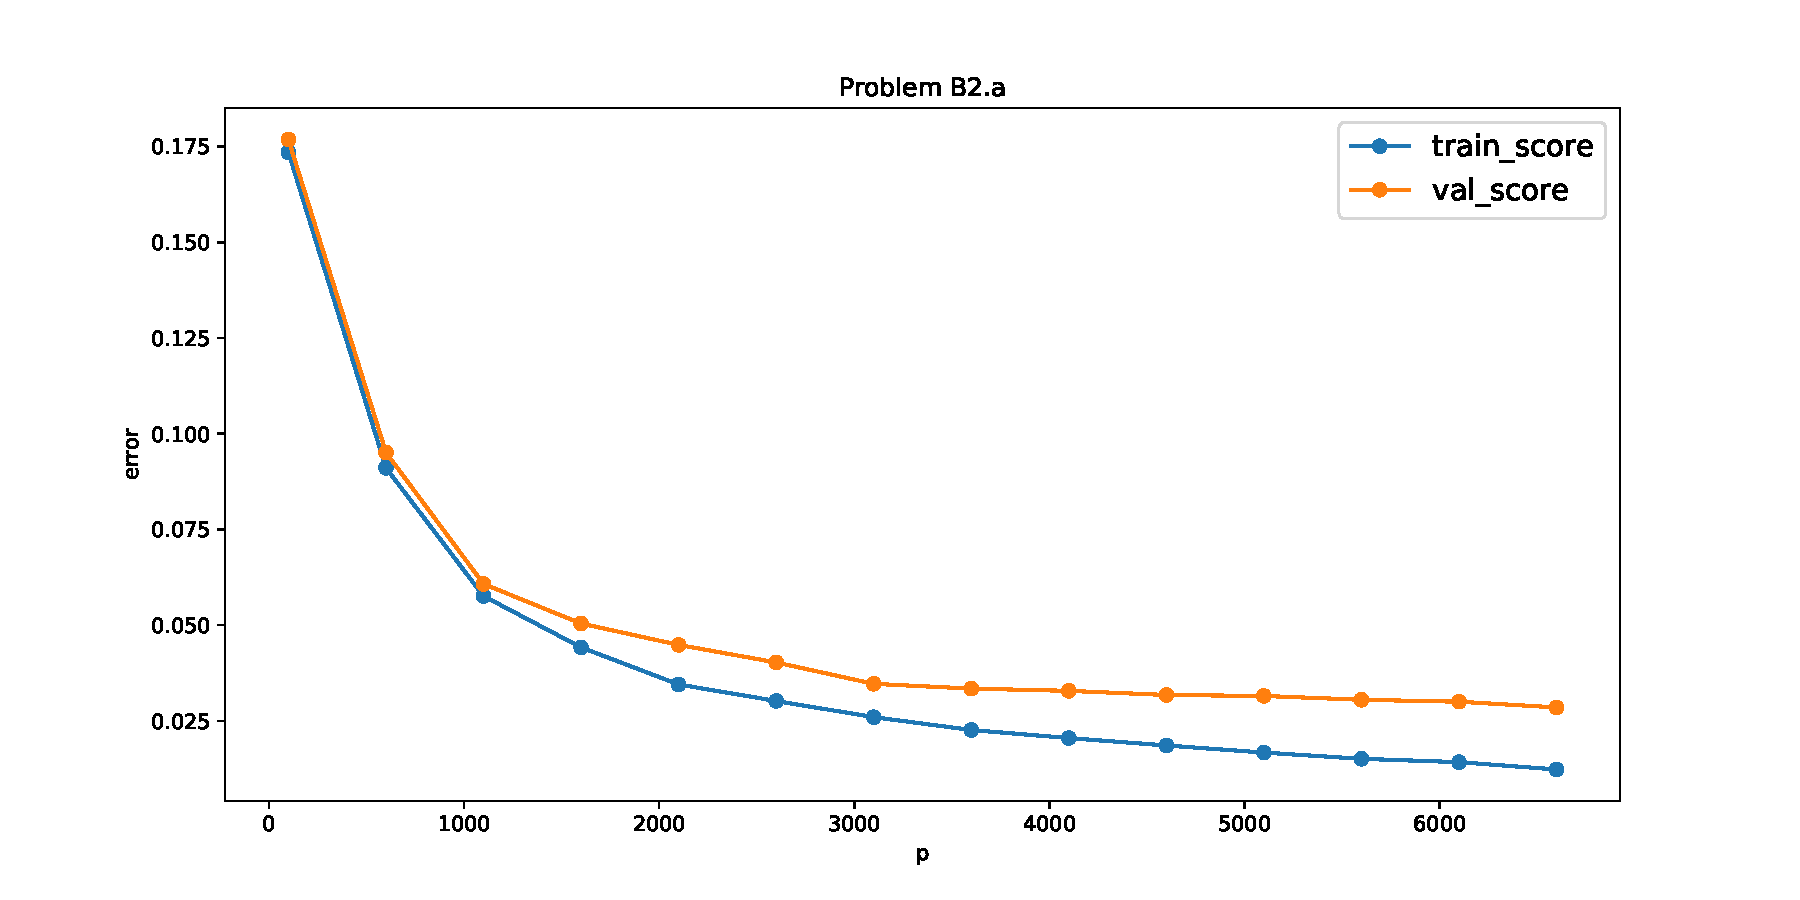
\includegraphics[width=0.9\textwidth]{code/b2_a.pdf}
            \caption{Problem B2.a}
            \label{figure:b2.a}
         \end{figure}
         
         \inputminted{python}{code/B2_a.py}
          \caption{Code for B2.a}
          \label{listing:b2.a}
    \item First, we compute the test error using the best $\widehat p$ (looking at the plot in a., we chose $\widehat p = 3100$), we obtain (the code is below):
    $$
    \Boxed{\widehat{\epsilon}_{\text{test}}(\widehat{f}) = 0.0348.}
    $$
    Now, $X_i$ from the Hoeffding's inequality are iid indicator variables taking values in $\{0,1\}$ corresponding to the $i$-th test example being classified correctly or not, respectively. So, to obtain the confidence interval, we plug in: $\delta = 0.05, m = 10000 \text{ (test set size)}, a=0, b=1$. Finally, we obtain $\sqrt{\frac{(b-a)^2 \log(2/\delta)}{2m}} \approx 0.01358102$ and
    $$
    \P \left( \left|\widehat{\epsilon}_{\text{test}}(\widehat{f})  - \epsilon(\widehat{f}) \right| \geq 0.01358102 \right)
                \leq 0.05,
    $$
    so the $95\%$ CI for $\epsilon(\widehat{f})$ is  $\boxed{0.0348 \pm 0.01358102}$ $\Box$.
    This question uses the same functions defined in the code for part a. and computes the test error as follows:
    \inputminted{python}{code/B2_b.py}
    
\end{enumerate}
\noindent\rule{\textwidth}{1pt}

\end{document}
